\documentclass[12pt, a4paper]{article}
\usepackage{graphicx}
\usepackage[section]{placeins}
\usepackage{float}
\usepackage[margin=1in]{geometry}
\usepackage{setspace}
\usepackage{fontspec}
\usepackage{cite}
\usepackage{indentfirst}

\setmainfont{Times New Roman}
\singlespace

\title{This Is A Test Title Of COMP90020 Term Project}
\author{Boyang Yue \\987093 \and Jing Wang \\1094546 \and Mengyang Chen \\1026634 \and Shuzhi Gong \\1047975 }
\date{}

\begin{document}

\maketitle

\begin{abstract}

This is abstract content. This is abstract content. This is abstract content. This is abstract content. This is abstract content. This is abstract content. This is abstract content. This is abstract content. This is abstract content. This is abstract content. This is abstract content. This is abstract content. This is abstract content. 

\noindent
\textit{\textbf{Keywords: } key1; key2; key3; key4; key5.}

\end{abstract}


\section{Introduction}

This is just a pic example. This is just a pic example. This is just a pic example. This is just a pic example. This is just a pic example. This is just a pic example. This is just a pic example. This is just a pic example. This is just a pic example. This is just a pic example. 

\begin{figure}[h!]
\centering
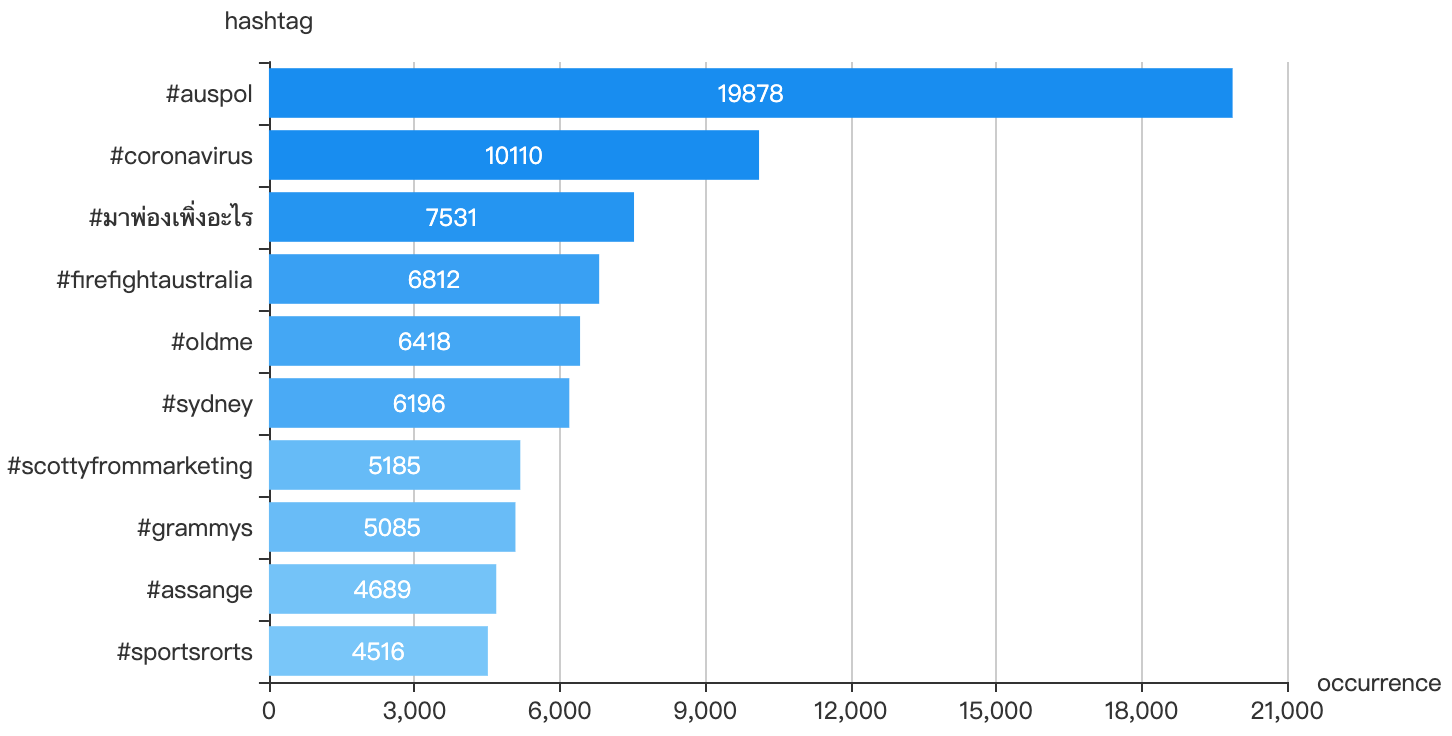
\includegraphics[width = 0.9\textwidth]{1.png}
\caption{Just a Test Pic}
\label{test}
\end{figure}


\section{Background Survey}

This is the paper in which RAFT has been proposed for the first time\cite{ongaro2014search}.

This is a paper about peer-to-peer file sharing systems\cite{saroiu2001measurement}.

\section{Comparative Analysis}


\section{Discussions}

\subsection{Future Directions}

\subsection{Application Domains}


\section{Algorithm}

\subsection{Advantages}

\subsection{Disadvantages}

\subsection{Implementation}





\newpage
\bibliography{refer.bib}
\bibliographystyle{ieeetr}


\end{document}